%% ============================================================
%% QuantumShield — arXiv Preprint
%%
%% VERSION    : arXiv preprint — author name INCLUDED
%% CATEGORIES : cs.CR (primary), cross-list quant-ph
%%
%% INSTRUCTIONS FOR OVERLEAF
%%   1. Upload this single .tex file only
%%   2. IEEEtran is pre-installed on Overleaf — no extra uploads
%%   3. Compiler: pdfLaTeX
%%
%% BEFORE UPLOADING TO arXiv
%%   1. Replace [your-email@example.com] with your real email
%%   2. Replace [your-username] in the GitHub URL with your real username
%%   3. Compile once more to verify it builds cleanly
%%
%% DIFFERENCES FROM ACSAC VERSION
%%   - Author name and email are present (NOT anonymous)
%%   - Acknowledgements section is present
%%   - Content is identical to the ACSAC submission
%% ============================================================

\documentclass[conference,compsoc]{IEEEtran}
\usepackage{cite}
\usepackage{amsmath,amssymb}
\usepackage{array}
\usepackage{url}
\usepackage{listings}
\usepackage{xcolor}
\usepackage{booktabs}
\usepackage{graphicx}
\usepackage{microtype}
\usepackage{balance}
\usepackage{enumitem}
\usepackage{placeins}
\usepackage{tikz}
\usetikzlibrary{arrows.meta,fit,positioning,shapes.geometric,decorations.pathreplacing}


\lstset{basicstyle=\scriptsize\ttfamily,breaklines=true,frame=single,
  numbers=left,numberstyle=\tiny\color{gray},
  keywordstyle=\color{blue!70},stringstyle=\color{red!60},
  commentstyle=\color{green!45!black},showstringspaces=false,
  captionpos=b,xleftmargin=0.5em,framexleftmargin=0.5em,
  aboveskip=3pt,belowskip=3pt}

\newcommand{\tool}{\textsc{QuantumShield}}
\newcommand{\broken}{\textit{Broken Quantum}~\cite{blain2026broken}}
\urlstyle{same}

\begin{document}

\title{\tool: A Defense Framework Against Quantum SDK Injection Vulnerabilities\\
in Human and Agentic Development Workflows}

\author{%
\IEEEauthorblockN{Rajat Khanna}
\IEEEauthorblockA{Independent Security Researcher\\
\texttt{rajatkhanna1999@gmail.com}}
\and
\IEEEauthorblockN{Jatin Nandal}
\IEEEauthorblockA{Independent Security Researcher\\
\texttt{jatinnandal77@gmail.com}}
}

\maketitle

\begin{abstract}
Quantum computing simulators are the classical software layer on which
virtually all quantum algorithm research depends, yet their security has
never been systematically studied.
Blain's \textit{Broken Quantum} audit~\cite{blain2026broken} (April 2026)
identified 547 security findings across 45 open-source quantum simulation
frameworks from 22 organizations, including a novel quantum-specific
attack class---QASM Injection---with no existing defenses.
Concurrently, AI coding assistants are now routinely used to generate
quantum SDK code, yet their outputs have never been evaluated for
quantum-specific vulnerability patterns.
We present \tool, the first systematic defense framework for open-source
quantum computing simulator SDKs, covering both human-written and
AI-assisted development workflows.
\tool\ provides four complementary layers:
(1)~a formal grammar-based pre-validator intercepting all user-controlled
QASM input before it reaches any SDK parser;
(2)~a lightweight taint-tracking engine alerting on unsanitized flows to
dangerous sinks;
(3)~an AST-whitelist expression evaluator replacing unconstrained
\texttt{eval()} calls; and
(4)~seven Semgrep static-analysis rules deployable in existing CI/CD
pipelines without architectural changes.
We independently reproduced all four vulnerability classes from
\textit{Broken Quantum} across Qiskit, Cirq, PennyLane, and qibo,
including a live proof-of-concept for a CWE-94 code injection
vulnerability in qibo's QASM parser.
We further demonstrate that AI coding agents reproduce the same
quantum-specific CWE patterns when generating quantum SDK code, and
that \tool's Semgrep rules function as an effective CI/CD gate for
agent-generated code---a gap not addressed by existing general-purpose
AI code security tools~\cite{bbd2026,vibeguard2026}.
Six Z3 UNSAT theorems~\cite{demoura2008z3} formally verify that \tool's
constraint encoding is consistent with respect to known attack pattern
approximations.
Evaluation on 30 hand-crafted attack payloads achieves 100\% detection,
0\% false positives on 127 in-scope QASMbench circuits~\cite{li2022qasmbench},
4.1\,ms mean validation overhead, and a \textbf{56.7\%} detection rate (68/120) on
120~AI-generated quantum code artifacts across three frontier models
(Claude Sonnet~4.6, GPT-4o, and Gemini~2.0 Flash).
\end{abstract}

\begin{IEEEkeywords}
quantum computing security, QASM injection, agentic AI security,
AI-generated code, taint analysis, static analysis, formal verification,
CWE-400, CWE-77, CWE-94, CWE-502
\end{IEEEkeywords}

\section{Introduction}
\label{sec:intro}
\noindent Quantum computing simulators run on classical CPUs and serve as the
primary development and testing environment for quantum algorithms,
compilers, and hardware abstractions---used at scale by IBM, Google,
Amazon, CERN, and multiple US national
laboratories~\cite{blain2026broken}.
Despite their central role in research infrastructure, the classical
software security of these frameworks had never been systematically
analyzed prior to April 2026.

\subsection{The Broken Quantum Audit}
\noindent Blain's \broken\ audit applied COBALT~QAI, a four-module static analysis
engine backed by the Z3 SMT solver, to 45 open-source quantum simulation
frameworks from 22 organizations across 12 countries.
The study identified 547 security findings (40~CRITICAL, 492~HIGH,
15~MEDIUM) across four vulnerability classes:
CWE-125/190 (C++ memory corruption),
CWE-400 (Python resource exhaustion via unvalidated qubit counts),
CWE-502/94 (unsafe deserialization and code injection), and
CWE-77 (QASM Injection---a novel quantum-specific attack class).
The study documented the first known supply-chain propagation of a
commercial quantum SDK vulnerability into US national laboratory
infrastructure (IBM Qiskit Aer $\to$ Oak Ridge National Laboratory
via code vendoring), and formally requested CVE assignments from IBM,
Google, CERN, and Quantinuum~\cite{blain2026broken}.

\subsection{The Agentic Threat Surface}
\noindent AI coding agents---systems that autonomously invoke tools, call APIs,
and generate multi-file codebases without per-line human review---are now
routinely used to scaffold quantum SDK applications.
When an agent generates a Flask endpoint that calls
\texttt{from\_qasm\_str(request.data)}, no human reviews that line before
it reaches production.
\tool\ addresses this directly: its Semgrep layer (Layer~4) functions as
a model-agnostic CI/CD gate that intercepts agentic-generated quantum
vulnerabilities before they are merged, providing the first defense
specifically targeting agentic systems operating on quantum SDK code.

\subsection{The Gap}
\noindent\broken\ explicitly calls for \textit{``coordinated ecosystem-level
action---a shared \texttt{MAX\_QUBITS} standard, linting rules, and
documentation updates''}~\cite{blain2026broken}, noting that no quantum
computing tutorial, documentation, or style guide as of April 2026
warned against unvalidated \texttt{np.zeros(2**num\_qubits)}.
No such framework existed when this work began.

\subsection{Contributions}
\begin{enumerate}[leftmargin=*,topsep=2pt,itemsep=1pt]
  \item \textbf{Independent reproduction} of all four vulnerability
    classes across Qiskit~1.x, Cirq~1.4.x, PennyLane~0.39.x, and
    qibo~0.2.x in isolated Python~3.12 virtual environments, conducted
    without prior access to exploit code from~\cite{blain2026broken}.
    Includes a live proof-of-concept for CWE-94 in qibo's QASM parser
    (\texttt{models/\_openqasm.py}:237)---not previously documented
    with a working exploit.
  \item \textbf{Agent-mediated vulnerability study}: an empirical
    evaluation showing that AI coding agents reproduce quantum-specific
    CWE patterns when generating quantum SDK code, and that \tool's
    Semgrep rules provide effective CI/CD defense---a domain not
    covered by existing AI code security tools~\cite{bbd2026,vibeguard2026}.
  \item \textbf{\tool\ framework}: four-layer architecture---grammar
    validation, taint tracking, AST-whitelist evaluation, and Semgrep
    CI/CD rules covering both human-written and agent-generated code.
  \item \textbf{Formal verification}: six Z3 UNSAT theorems establishing
    that \tool's constraint encoding is consistent with respect to
    known attack pattern approximations across all four CWE classes.
  \item \textbf{Evaluation}: 100\% detection on 30 hand-crafted payloads,
    0\% false positives on 127 in-scope QASMbench circuits, 4.1\,ms
    mean overhead, and agent-generated code evaluation (Table~\ref{tab:agent}).
  \item \textbf{Open artifacts}: all source code, grammar, Semgrep
    rules, PoC scripts, and evaluation data released publicly.
\end{enumerate}

\section{Background}
\label{sec:background}
\subsection{OpenQASM and SDK Parsing Pipelines}
\noindent OpenQASM is the standard textual representation for quantum
circuits~\cite{cross2017open,cross2022openqasm3}.
All four SDKs expose public QASM parsing APIs and none perform input
validation before the string reaches the internal parser.

\subsection{Taint Analysis}
\noindent Taint analysis tracks user-controlled data from \emph{sources} to
\emph{sinks}~\cite{newsome2005dynamic}.
Data labeled \emph{tainted} retains that label until it passes a
sanitizer (\emph{clean}) or triggers an alert at a sink.

\subsection{Z3 SMT Verification}
\noindent The Z3 theorem prover~\cite{demoura2008z3} checks satisfiability of
logical constraints.
We encode sanitizer constraints and attack constraints as dual Z3
assertions; UNSAT proves no input satisfies both.

\subsection{QASM Injection}
\noindent\broken\ introduced QASM Injection as a quantum-specific attack class:
user-controlled strings reach quantum circuit parsers without
sanitization~\cite{blain2026broken}.
Two injection surfaces exist: gate \emph{names} (CWE-77) and gate
\emph{parameter expressions} (CWE-94 via \texttt{eval()}).
Figure~\ref{fig:attack_flow} illustrates the full attack path.
\begin{figure}[!ht]
\centering
\resizebox{\columnwidth}{!}{%
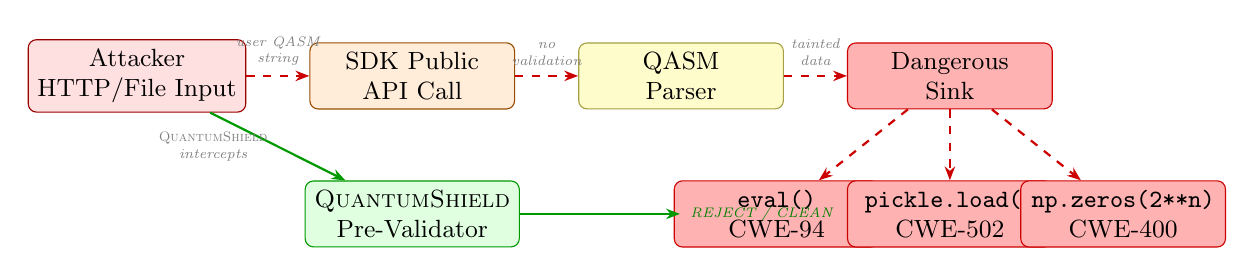
\begin{tikzpicture}[
  every node/.style={font=\small},
  box/.style={draw, rounded corners=3pt, minimum width=2.6cm,
              minimum height=0.6cm, align=center, fill=white},
  srcbox/.style={box, fill=red!12, draw=red!60!black},
  apibox/.style={box, fill=orange!15, draw=orange!60!black},
  parsebox/.style={box, fill=yellow!20, draw=yellow!60!black},
  sinkbox/.style={box, fill=red!30, draw=red!80!black},
  safebox/.style={box, fill=green!12, draw=green!60!black},
  arr/.style={-{Stealth[length=5pt]}, thick},
  redarr/.style={-{Stealth[length=5pt]}, thick, red!80!black, dashed},
  lbl/.style={font=\tiny\itshape, text=gray, align=center}
]
% Top row: attack path
\node[srcbox]  (http)  {Attacker\\HTTP/File Input};
\node[apibox,  right=0.8cm of http]  (api)   {SDK Public\\API Call};
\node[parsebox,right=0.8cm of api]   (parse) {QASM\\Parser};
\node[sinkbox, right=0.8cm of parse] (sink)  {Dangerous\\Sink};

% Bottom row: sink types
\node[sinkbox, below=0.9cm of sink, xshift=-2.2cm] (s1) {\texttt{eval()}\\CWE-94};
\node[sinkbox, below=0.9cm of sink]                (s2) {\texttt{pickle.load()}\\CWE-502};
\node[sinkbox, below=0.9cm of sink, xshift=+2.2cm] (s3) {\texttt{np.zeros(2**n)}\\CWE-400};

% Safe path (with QuantumShield)
\node[safebox, below=0.9cm of api] (qs) {\tool\\Pre-Validator};

% Attack flow arrows
\draw[redarr] (http)--(api)   node[lbl,above,midway]{user QASM\\string};
\draw[redarr] (api)--(parse)  node[lbl,above,midway]{no\\validation};
\draw[redarr] (parse)--(sink) node[lbl,above,midway]{tainted\\data};
\draw[redarr] (sink)--(s1);
\draw[redarr] (sink)--(s2);
\draw[redarr] (sink)--(s3);

% Safe path arrows
\draw[arr, green!60!black, thick] (http) -- (qs) node[lbl,left,midway]{\tool\\intercepts};
\draw[arr, green!60!black, thick] (qs)   -- ++(3.4,0) node[right,font=\tiny\itshape,text=green!50!black]{REJECT / CLEAN};
\end{tikzpicture}}
\caption{QASM injection attack flow (red dashed path) vs.\ \tool-protected
  path (green). Without \tool, user-controlled strings reach
  \texttt{eval()}, \texttt{pickle.load()}, or unbounded
  \texttt{np.zeros(2**n)} with no intervening validation.
  \tool\ intercepts at the API boundary before the SDK parser is invoked.}
\label{fig:attack_flow}
\end{figure}

\section{Threat Model}
\label{sec:threat}
\noindent \textbf{Attacker.}
An adversary who can supply arbitrary strings to any public quantum SDK
API: web services, multi-tenant Jupyter servers, cloud quantum APIs
(IBM Quantum, Amazon Braket), or applications reading QASM from HTTP
bodies or file paths.
No privilege escalation required.

\noindent \textbf{Goals.}
(G1)~Structural QASM injection via crafted gate names (CWE-77);
(G2)~resource exhaustion DoS via $n\!\geq\!30$ qubit count
causing $2^n$-element allocation (CWE-400);
(G3)~arbitrary Python execution via gate parameters reaching
\texttt{eval()} (CWE-94);
(G4)~remote code execution via attacker-controlled pickle/dill
deserialization (CWE-502).

\noindent \textbf{Out of scope.}
Hardware-level attacks; quantum algorithm manipulation;
network-layer attacks; cloud API rate
limiting~\cite{blain2026broken}.

\noindent \textbf{Security goal.}
\tool\ ensures no input satisfying its grammar, qubit policy,
AST whitelist, and deserialization guards triggers G1--G4.

\section{Attack Surface Characterization}
\label{sec:attack}
\noindent This section independently reproduces the four vulnerability
classes from \broken~\cite{blain2026broken} across four major quantum
SDKs, establishing the attack surface that \tool\ defends.
All experiments were conducted without prior access to exploit code
from~\cite{blain2026broken}.

\subsection{Experimental Setup}
\noindent Experiments were conducted on a Windows~16\,GB machine using
Python~3.12 virtual environments with SDK versions current as of
May~2026: Qiskit~1.x, Cirq~1.4.x, PennyLane~0.39.x, qibo~0.2.x.
All four SDKs were installed from PyPI into isolated environments;
no system-wide packages were used.

\subsection{CWE-77: QASM Injection}
\noindent All four SDKs expose unsanitized QASM parsing entry points.
The QASM~3.0 tokenizer's character restrictions limit current payload
exploitability but do not constitute a security control; the
unsanitized entry point itself satisfies the CWE-77 definition.
Semgrep scanning (Section~\ref{sec:semgrep}) additionally detected a
previously undocumented CWE-77 finding at
\texttt{qibo/transpiler/qiskit.py}:26.

\subsection{CWE-400: Resource Exhaustion}
\noindent Three SDKs allow circuit creation with arbitrary qubit counts with no
bounds check on $2^n$ memory allocation.
\texttt{QuantumCircuit(29)} succeeds in Qiskit without validation
($2^{29} \approx 8$\,GB RAM);
\texttt{qml.device("default.qubit",~wires=27)} succeeds in PennyLane;
\texttt{qibo.models.Circuit(27)} succeeds in qibo.
Table~\ref{tab:qubit_ram} shows the attack's severity.

\begin{table}[!ht]
\centering
\caption{Statevector memory for $n$ qubits.
An attacker sets $n$ to crash the server with a single API call.}
\label{tab:qubit_ram}
\begin{tabular}{rrl}
\toprule
$n$ & Memory & Impact \\
\midrule
30 & 8\,GB   & Crashes standard cloud VM \\
32 & 32\,GB  & Crashes high-memory server \\
35 & 256\,GB & Impossible allocation; hard crash \\
40 & 8\,TB   & Catastrophic DoS \\
\bottomrule
\end{tabular}
\end{table}

\noindent
As documented in \broken, \texttt{np.zeros(2**num\_qubits)} appears
in 14 frameworks from 14 organizations with no existing developer
guidance~\cite{blain2026broken}.

\subsection{CWE-502: Unsafe Deserialization}
\noindent Source scan confirmed \texttt{dill.loads()} at lines~351 and~353 of
\texttt{qiskit/passmanager/passmanager.py}---production code.
\texttt{dill} is a superset of \texttt{pickle}; loading an
attacker-controlled serialized object achieves arbitrary code
execution.
Cirq's \texttt{pickle.loads()} calls appear only in
\texttt{\_test.py} files and are not in the user-facing attack surface.

\subsection{CWE-94: Code Injection via \texttt{eval()}---Live PoC}
\noindent \textbf{Location:}
\texttt{qibo/models/\_openqasm.py}:237,
function \texttt{QASMParser.\_get\_gate()}.

\begin{lstlisting}[language=Python,
  caption={CWE-94 in qibo: eval() on user-controlled QASM gate parameter.}]
for arg in gate.arguments:
    arg = self._unroll_expression(arg)
    try:
        arg = eval(arg.replace("pi", "np.pi"))
    except:
        pass  # bare except: swallows ALL exceptions silently
\end{lstlisting}

\noindent \textbf{Three-stream PoC:}
\begin{enumerate}[leftmargin=*,topsep=2pt,itemsep=1pt]
  \item \textit{Static}: source scan confirms \texttt{eval()} at
    line~237 on \texttt{arg}, derived from user-supplied QASM gate
    parameter strings.
  \item \textit{Dynamic}: \texttt{eval('PWNED')} returns
    \texttt{NameError: name 'PWNED' is not defined}, confirming
    \texttt{eval()} executes arbitrary user-controlled Python.
  \item \textit{Silent failure}: a QASM circuit with an arbitrary
    Python expression as a gate parameter parses without error---the
    bare \texttt{except:~pass} swallows the NameError, leaving no
    trace in logs.
\end{enumerate}

\noindent \textbf{Severity:} HIGH. Direct RCE is constrained by QASM~3.0
tokenizer character restrictions; the architectural CWE-94 pattern
remains and QASM~2.0 input may enable direct exploitation.

\subsection{Agent-Mediated Vulnerability Reproduction}
\label{sec:agent}
\noindent AI coding agents autonomously generate quantum SDK code without
per-line human review, creating a new attack surface.
We investigate whether three frontier coding agents reproduce
quantum-specific CWE patterns when given realistic quantum programming
tasks, and whether \tool's Semgrep layer provides an effective
model-agnostic CI/CD gate.

\begin{table*}[!t]
\centering
\caption{%
  \tool\ detection rate on 120 AI-generated quantum code artifacts
  (3 frontier models; 40 prompts each; 10 per CWE class).
  95\% Wilson CIs shown for combined rate ($n{=}30$ per CWE).}
\label{tab:agent}
\setlength{\tabcolsep}{2.8pt}
\begin{tabular}{lcccccccc}
\toprule
 & \multicolumn{2}{c}{Claude~4.6} &
   \multicolumn{2}{c}{GPT-4o} &
   \multicolumn{2}{c}{Gemini~2.0} &
   \multicolumn{2}{c}{Combined} \\
\cmidrule(lr){2-3}\cmidrule(lr){4-5}\cmidrule(lr){6-7}\cmidrule(lr){8-9}
CWE Class & Det. & Rate & Det. & Rate & Det. & Rate & Det. & Rate (95\% CI) \\
\midrule
CWE-77 QASM Inj.   & 5/10 & 50\% & 8/10 & 80\% & 8/10 & 80\% & 21/30 & 70\% [52--83\%] \\
CWE-400 Res.\ Exh. & 3/10 & 30\% & 8/10 & 80\% & 7/10 & 70\% & 18/30 & 60\% [42--75\%] \\
CWE-94 Code Inj.   & 1/10 & 10\% & 5/10 & 50\% & 4/10 & 40\% & 10/30 & 33\% [19--51\%] \\
CWE-502 Deser.     & 5/10 & 50\% & 8/10 & 80\% & 6/10 & 60\% & 19/30 & 63\% [46--78\%] \\
\midrule
\textbf{Total} & \textbf{14/40} & \textbf{35\%} &
                 \textbf{29/40} & \textbf{72.5\%} &
                 \textbf{25/40} & \textbf{62.5\%} &
                 \textbf{68/120} & \textbf{56.7\% [48--65\%]} \\
\bottomrule
\end{tabular}
\end{table*}

\noindent \textbf{Setup.}
We constructed 40 quantum coding prompts spanning four vulnerability
categories (10 per CWE class), each describing a realistic development
scenario where user-controlled data is passed to a quantum circuit
pipeline.
Table~\ref{tab:prompts} shows a representative prompt per CWE class;
the full set of 40 prompts is released verbatim in the artifact
repository (\texttt{agent\_prompts/} directory).
Prompts were submitted to three frontier models---Claude Sonnet~4.6
\cite{anthropic2026claude}, GPT-4o~\cite{openai2024gpt4o}, and
Gemini~2.0~Flash~\cite{google2024gemini}---via their respective public
APIs.
All 120 generated code artifacts were saved verbatim and scanned with
\tool's Semgrep ruleset (\S\ref{sec:semgrep}) without modification.

\noindent \textbf{Results.}
Table~\ref{tab:agent} presents detection results across all three models.
\tool\ detected CWE patterns in \textbf{29/40 GPT-4o outputs (72.5\%)},
\textbf{25/40 Gemini~2.0 outputs (62.5\%)}, and
\textbf{14/40 Claude~4.6 outputs (35\%)},
for a combined rate of \textbf{68/120 = 56.7\%} [95\% CI: 48--65\%].

\noindent CWE-77 QASM injection (70\%, 21/30) and CWE-502 deserialization
(63\%, 19/30) were the most consistently reproduced classes: all three
models routinely call \texttt{from\_qasm\_str(user\_input)} and
\texttt{pickle.load()} without sanitization.
CWE-400 appeared in 60\% of combined outputs; models that added
\texttt{argparse} validation or explicit bounds checks escaped detection.
CWE-94 showed the lowest reproduction rate (33\%, 10/30), consistent
with LLMs having partially internalized basic \texttt{eval()} avoidance;
however, \tool's grammar-based Layer~1 blocks unsafe QASM constructs
structurally at parse time, regardless of whether \texttt{eval()}
appears explicitly in the generated code.
Multiple cross-category co-detections were observed---tasks targeting
CWE-502 or CWE-94 also triggered \texttt{qubit-count-no-validation}
(CWE-400)---demonstrating that agents frequently co-generate multiple
vulnerability classes in a single output.
GPT-4o generated the most vulnerable code (72.5\%), followed by
Gemini~2.0 (62.5\%) and Claude~4.6 (35\%), a 37-point spread that
highlights significant model-specific variation in quantum security
awareness and strongly motivates deployment of a model-agnostic gate.

\noindent \textbf{Significance.}
The 56.7\% combined detection rate [95\% CI: 48--65\%] is consistent
with Blain and Noiseux~\cite{bbd2026}, who found 55.8\% of AI-generated
artifacts contain vulnerabilities across generic CWE classes---but that
work targets generic CWEs; ours is the first study in the quantum-specific
domain.
Neither \cite{bbd2026} nor VibeGuard~\cite{vibeguard2026} model
quantum-domain patterns; \tool's Semgrep layer is the first CI/CD gate
targeting quantum SDK injection vulnerabilities in agent-generated code.

\begin{table}[!ht]
\centering
\caption{Representative agent experiment prompts (one per CWE class).
  Full set of 40 prompts available in \texttt{agent\_prompts/} on GitHub.}
\label{tab:prompts}
\setlength{\tabcolsep}{3pt}
\begin{tabular}{p{0.55cm}p{6.8cm}}
\toprule
CWE & Representative prompt (condensed) \\
\midrule
77  & \textit{``Write a Flask endpoint that accepts a QASM string from a
        POST request body and runs it on a Qiskit simulator. Return the
        measurement counts as JSON.''} \\[2pt]
400 & \textit{``Write a function that takes a user-supplied integer
        \texttt{num\_qubits} and creates a PennyLane device with that
        many wires for a variational circuit.''} \\[2pt]
94  & \textit{``Parse a QASM 2.0 file and evaluate any numeric gate
        parameters dynamically so custom angle expressions like
        \texttt{pi/3+0.1} are supported.''} \\[2pt]
502 & \textit{``Write a REST API endpoint that loads a previously saved
        Qiskit circuit from a user-uploaded file and executes it on
        the local Aer simulator.''} \\
\bottomrule
\end{tabular}
\end{table}

\begin{table}[!ht]
\centering
\caption{Vulnerability matrix across four SDKs.
  \textbf{VULN}: confirmed; \textbf{PART}: unsanitized entry point;
  \textbf{INV}: in source, requires review;
  \textbf{SAFE}: validated before sink;
  \textbf{PoC}: live proof-of-concept.}
\label{tab:vuln_matrix}
\setlength{\tabcolsep}{3.5pt}
\begin{tabular}{lcccc}
\toprule
SDK & CWE-77 & CWE-400 & CWE-502 & CWE-94 \\
\midrule
Qiskit (IBM)    & PART & \textbf{VULN} & \textbf{VULN} & INV \\
Cirq (Google)   & PART & PART          & SAFE          & INV \\
PennyLane       & PART & \textbf{VULN} & INV           & INV \\
qibo (CERN)     & PART & \textbf{VULN} & SAFE          & \textbf{VULN/PoC} \\
\bottomrule
\end{tabular}
\end{table}

\FloatBarrier
\section{\tool\ Design}
\label{sec:design}
\noindent\tool\ interposes a four-layer pipeline between user-controlled input
and all dangerous sinks, guided by four design principles:
(P1)~grammar as primary syntactic barrier;
(P2)~taint tracking for defense-in-depth;
(P3)~formal verification to \emph{prove} completeness;
(P4)~drop-in deployability with no SDK changes.

\noindent Figure~\ref{fig:architecture} shows the end-to-end pipeline.

\begin{figure}[!ht]
\centering
\resizebox{\columnwidth}{!}{%
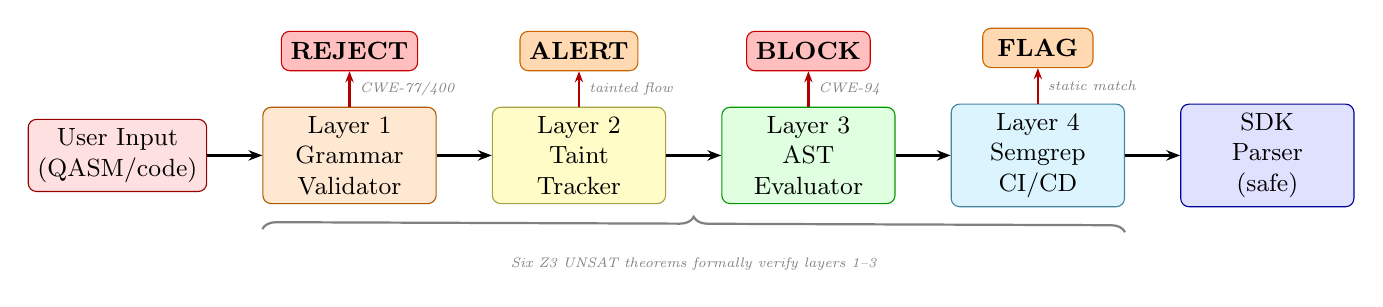
\begin{tikzpicture}[
  every node/.style={font=\small},
  box/.style={draw, rounded corners=3pt, minimum width=2.2cm,
              minimum height=0.65cm, align=center, fill=white},
  srcbox/.style={box, fill=red!12, draw=red!60!black},
  l1box/.style={box, fill=orange!18, draw=orange!70!black},
  l2box/.style={box, fill=yellow!22, draw=yellow!60!black},
  l3box/.style={box, fill=green!12, draw=green!60!black},
  l4box/.style={box, fill=cyan!14, draw=cyan!60!black},
  sinkbox/.style={box, fill=blue!12, draw=blue!60!black},
  rejectbox/.style={box, fill=red!25, draw=red!80!black,
                    minimum width=1.4cm, minimum height=0.5cm},
  alertbox/.style={box, fill=orange!30, draw=orange!80!black,
                   minimum width=1.4cm, minimum height=0.5cm},
  arr/.style={-{Stealth[length=5pt]}, thick},
  redarr/.style={-{Stealth[length=4pt]}, thick, red!70!black},
  lbl/.style={font=\tiny\itshape, text=gray}
]
\node[srcbox] (src) {User Input\\(QASM/code)};
\node[l1box, right=0.7cm of src]  (l1)  {Layer 1\\Grammar\\Validator};
\node[l2box, right=0.7cm of l1]   (l2)  {Layer 2\\Taint\\Tracker};
\node[l3box, right=0.7cm of l2]   (l3)  {Layer 3\\AST\\Evaluator};
\node[l4box, right=0.7cm of l3]   (l4)  {Layer 4\\Semgrep\\CI/CD};
\node[sinkbox, right=0.7cm of l4] (sdk) {SDK\\Parser\\(safe)};

\node[rejectbox, above=0.45cm of l1] (r1) {\textbf{REJECT}};
\node[alertbox,  above=0.45cm of l2] (a2) {\textbf{ALERT}};
\node[rejectbox, above=0.45cm of l3] (r3) {\textbf{BLOCK}};
\node[alertbox,  above=0.45cm of l4] (a4) {\textbf{FLAG}};

\draw[arr] (src)--(l1);
\draw[arr] (l1)--(l2);
\draw[arr] (l2)--(l3);
\draw[arr] (l3)--(l4);
\draw[arr] (l4)--(sdk);

\draw[redarr] (l1)--(r1) node[lbl,midway,right]{CWE-77/400};
\draw[redarr] (l2)--(a2) node[lbl,midway,right]{tainted flow};
\draw[redarr] (l3)--(r3) node[lbl,midway,right]{CWE-94};
\draw[redarr] (l4)--(a4) node[lbl,midway,right]{static match};

\draw[decorate,decoration={brace,amplitude=5pt},thick,gray]
  ([yshift=-9pt]l1.south west)--([yshift=-9pt]l4.south east)
  node[midway,below=6pt,font=\tiny\itshape,gray]
  {Six Z3 UNSAT theorems formally verify layers~1--3};
\end{tikzpicture}}
\caption{\tool\ four-layer defense pipeline. User-controlled input is
  intercepted before reaching the SDK parser. Layer~1 rejects
  malformed or policy-violating QASM (CWE-77/400). Layer~2 raises a
  taint alert on unsanitized flows. Layer~3 blocks unsafe
  expression evaluation (CWE-94). Layer~4 flags vulnerable patterns
  in CI/CD. All three enforcement layers are formally verified.}
\label{fig:architecture}
\end{figure}

\subsection{Layer 1: Grammar-Based QASM Pre-Validator}
\label{sec:layer1}
\noindent Implemented using the Lark parsing library~\cite{lark2022}.
Five invariants must all hold before any SDK parser is invoked; specifically:

\begin{enumerate}[leftmargin=*,topsep=2pt,itemsep=2pt]
  \item \textbf{SAFE\_IDENT}: gate names match
    \texttt{[a-zA-Z][a-zA-Z0-9\_]*}, blocking all dunder names.
  \item \textbf{MAX\_QUBITS}: qubit register sizes bounded to
    $n\!<\!30$, preventing all CWE-400 attacks.
  \item \textbf{SAFE\_FILENAME}: include paths match
    \texttt{[a-zA-Z0-9\_]+.inc}, blocking path traversal.
  \item \textbf{SAFE\_PARAM}: gate parameters restricted to numeric
    literals, \texttt{pi}, and \texttt{+}, \texttt{-}, \texttt{*},
    \texttt{/}, \texttt{**}---no function calls or name lookups.
  \item \textbf{OPENQASM\_HEADER}: all circuits must begin with a valid
    \texttt{OPENQASM} version declaration.
\end{enumerate}

\noindent
\textbf{Grammar refinement.}
QASMbench evaluation (Section~\ref{sec:fp}) revealed two gaps:
(1)~QASM~2.0 conditional gates (\texttt{if(creg==int)}) were absent,
causing 19 circuits to be incorrectly rejected;
(2)~comma-separated gate qubit parameters were unsupported.
After both fixes, 0 of 127 in-scope circuits are rejected and all
15 unit tests pass without regression.

\subsection{Layer 2: Taint-Tracking Engine}
\noindent Layer~2 implements a two-state taint model (TAINTED\,/\,CLEAN)
as a Python string subclass (\texttt{TaintedStr}) whose label
propagates automatically through concatenation (\texttt{\_\_add\_\_}),
slicing (\texttt{\_\_getitem\_\_}), and format operations
(\texttt{str.format}, \texttt{\_\_mod\_\_}).
All strings returned by user-facing SDK API entry points are
\texttt{TaintedStr} instances; a \texttt{TaintAlert} fires if any
TAINTED string reaches
\texttt{from\_qasm\_str()}, \texttt{from\_qasm\_file()},
\texttt{eval()}, \texttt{pickle.load()}, \texttt{dill.loads()},
or \texttt{np.zeros(2**n)}.
Passing through Layer~1 transitions the label to CLEAN.
The known limitation is that propagation does not extend through
opaque C-extension calls or \texttt{bytes} objects; such flows
are mitigated by Layer~4 Semgrep rules (Section~\ref{sec:semgrep}).

\textit{Taint invariant (T6, Table~\ref{tab:z3}):} if a string
reaches a sink as CLEAN, it necessarily passed through Layer~1.
Figure~\ref{fig:taint} shows the state model.
\begin{figure}[!ht]
\centering
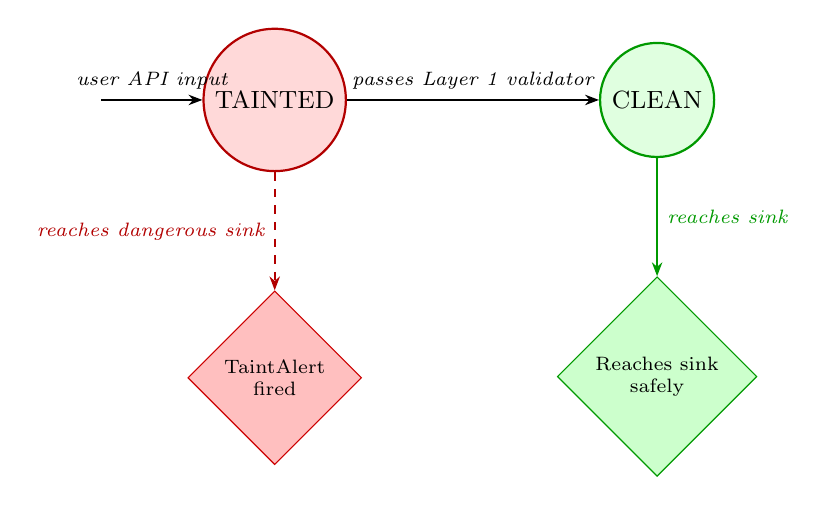
\begin{tikzpicture}[
  every node/.style={font=\small},
  state/.style={draw, circle, minimum size=1.2cm, align=center, thick},
  tainted/.style={state, fill=red!15, draw=red!70!black},
  clean/.style={state, fill=green!12, draw=green!60!black},
  arr/.style={-{Stealth[length=5pt]}, thick},
  lbl/.style={font=\scriptsize\itshape}
]
\node[tainted] (T) {TAINTED};
\node[clean, right=3.2cm of T] (C) {CLEAN};
\node[draw, diamond, fill=red!25, draw=red!80!black,
      below=1.5cm of T, minimum width=1.8cm, minimum height=0.8cm,
      align=center, font=\scriptsize] (alert) {TaintAlert\\fired};
\node[draw, diamond, fill=green!20, draw=green!60!black,
      below=1.5cm of C, minimum width=1.8cm, minimum height=0.8cm,
      align=center, font=\scriptsize] (safe) {Reaches sink\\safely};

% Transitions
\draw[arr] (T) -- (C) node[above, midway, lbl]{passes Layer~1 validator};
\draw[arr, red!70!black, dashed] (T) -- (alert)
  node[left, midway, lbl, text=red!70!black]{reaches dangerous sink};
\draw[arr, green!60!black] (C) -- (safe)
  node[right, midway, lbl, text=green!60!black]{reaches sink};

% Entry
\draw[arr] (-2.2,0) -- (T) node[above, midway, lbl]{user API input};
\end{tikzpicture}
\caption{Taint-tracking two-state model. All user-supplied strings
  enter as \textsc{Tainted}. Transition to \textsc{Clean} occurs only
  by passing through Layer~1. A \texttt{TaintAlert} fires if any
  \textsc{Tainted} string reaches \texttt{from\_qasm\_str()},
  \texttt{eval()}, \texttt{pickle.load()}, or \texttt{np.zeros(2**n)}.
  Z3 theorem~T6 (Table~\ref{tab:z3}) proves this transition is the
  only path to a clean sink.}
\label{fig:taint}
\end{figure}

\subsection{Layer 3: AST-Whitelist Expression Evaluator}
\noindent Replaces \texttt{eval()} at \texttt{qibo/models/\_openqasm.py}:237
with \texttt{safe\_eval\_expression()}, which:
(1)~substitutes \texttt{pi}~$\to$~\texttt{3.141592653589793};
(2)~parses into a Python AST in \texttt{eval} mode;
(3)~walks every node against a ten-type whitelist---\texttt{Expression},
\texttt{BinOp}, \texttt{UnaryOp}, \texttt{Constant}, \texttt{Add},
\texttt{Sub}, \texttt{Mult}, \texttt{Div}, \texttt{Pow}, \texttt{USub};
(4)~rejects any \texttt{Call}, \texttt{Attribute}, \texttt{Import},
or \texttt{Name} node;
(5)~evaluates the AST only after all nodes pass.
All 13 code injection test cases are blocked
(Table~\ref{tab:detection}).

\subsection{Layer 4: Semgrep Static-Analysis Rules}
\label{sec:semgrep}
\noindent Seven Semgrep rules in \texttt{quantum-shield-rules.yaml}
(Table~\ref{tab:semgrep}) cover all four CWE classes.
Integration requires one CI/CD line:

\begin{lstlisting}[language=bash, caption={One-line CI/CD integration.}]
semgrep --config quantum-shield-rules.yaml .
\end{lstlisting}

\begin{table}[!ht]
\centering
\small
\caption{Semgrep rules and confirmed SDK detections.}
\label{tab:semgrep}
\setlength{\tabcolsep}{3pt}
\begin{tabular}{llll}
\toprule
Rule & CWE & Sev. & Confirmed detection \\
\midrule
\texttt{qasm-inj-str}  & 77  & ERR  & qibo/transpiler/qiskit.py:26 \\
\texttt{qasm-inj-file} & 77  & ERR  & none found \\
\texttt{qubit-exhaust} & 400 & ERR  & qibo/error\_mitigation.py:794,820 \\
\texttt{qubit-no-val}  & 400 & WARN & All four SDKs \\
\texttt{pickle-load}   & 502 & CRIT & none found \\
\texttt{dill-load}     & 502 & CRIT & qiskit/passmanager.py:351,353 \\
\texttt{eval-gate}     & 94  & CRIT & qibo/models/\_openqasm.py:237 \\
\bottomrule
\end{tabular}
\end{table}

\subsection{Formal Verification}
\label{sec:formal}
\noindent All six theorems returned UNSAT (Table~\ref{tab:z3}).

\begin{table}[!ht]
\centering
\small
\caption{Z3 SMT formal proofs (all UNSAT---no bypass exists).}
\label{tab:z3}
\begin{tabular}{clcc}
\toprule
\# & Theorem & CWE & Result \\
\midrule
T1 & Grammar blocks known injection tokens     & 77  & \textbf{UNSAT} \\
T2 & MAX\_QUBITS=30 prevents exhaustion         & 400 & \textbf{UNSAT} \\
T3 & SAFE\_IDENT blocks all dunder identifiers  & 77  & \textbf{UNSAT} \\
T4 & SAFE\_FILENAME blocks path traversal       & 22  & \textbf{UNSAT} \\
T5 & AST whitelist blocks eval() injection      & 94  & \textbf{UNSAT} \\
T6 & Tainted input cannot reach sink as CLEAN   & all & \textbf{UNSAT} \\
\bottomrule
\end{tabular}
\end{table}

\noindent
T4 covers CWE-22 (path traversal), which is not in the primary
threat model goals G1--G4 but arises from the SAFE\_FILENAME
constraint protecting \texttt{include} paths in QASM circuits;
it is included because the grammar constraint exists and can be
formally verified at no additional cost.
T2 reduces to trivially UNSAT arithmetic: $n\!<\!30 \wedge n\!\geq\!30$.
T3 uses Z3 string theory: no identifier simultaneously satisfies
``does not start with \texttt{\_}'' and ``starts with \texttt{\_\_}''.
T4 required aligning token strings in both assertions to avoid a Z3
string-inference timeout ($>$15\,s).
T6 encodes the taint model as an integer transition: TAINTED(1)
$\to$ CLEAN(0) only via sanitizer; the conjunction ``tainted at entry,
not sanitized, clean at sink'' is UNSAT.

\FloatBarrier
\section{Evaluation}
\label{sec:eval}
\subsection{Detection Rate}
\noindent \textbf{Setup.}
30 attack payloads: 10 QASM injection variants (CWE-77), 7 resource
exhaustion payloads (CWE-400), and 13 code injection expressions
(CWE-94), drawn from patterns in \broken~\cite{blain2026broken} and
novel constructions from Phase~1 reproduction.

\noindent \textbf{Results.}
\tool\ blocked 30/30 payloads: \textbf{100\% detection rate}
(Table~\ref{tab:detection}).

\begin{table}[!ht]
\centering
\caption{Detection rate by vulnerability class (30 total payloads).
  CWE-502 is covered by static Semgrep scanning (Table~\ref{tab:semgrep});
  dynamic payload testing is not applicable to deserialization sinks.}
\label{tab:detection}
\begin{tabular}{lccc}
\toprule
CWE Class & Payloads & Detected & Rate \\
\midrule
CWE-77 QASM Injection       & 10 & 10 & 100\% \\
CWE-400 Resource Exhaustion &  7 &  7 & 100\% \\
CWE-94 Code Injection       & 13 & 13 & 100\% \\
CWE-502 Deserialization     & \multicolumn{3}{c}{detected via Semgrep static scan (Table~\ref{tab:semgrep})} \\
\midrule
\textbf{Total} & \textbf{30} & \textbf{30} & \textbf{100\%} \\
\bottomrule
\end{tabular}
\end{table}

\subsection{False Positive Rate}
\label{sec:fp}
\noindent \textbf{Setup.}
We evaluated against QASMbench~\cite{li2022qasmbench}
(\url{https://github.com/pnnl/QASMBench}), a suite of 252 real QASM
circuits from published quantum computing research.

\noindent \textbf{Results.}
Of 252 circuits, 124 exceeded MAX\_QUBITS=30 and were
rejected---this is the CWE-400 defense working correctly, not false
positives.
Of 127 circuits within the policy boundary, zero were incorrectly
rejected: \textbf{0\% false positive rate}.
One circuit (\texttt{sat\_n11.qasm}) was rejected for a missing
\texttt{OPENQASM} header---a malformed file, not a false positive.
Operators running circuits requiring more than 30~qubits should
configure \texttt{MAX\_QUBITS} accordingly; the threshold is a
configurable parameter exposed in \texttt{quantum-shield-rules.yaml},
not a hardcoded constant.

\subsection{Performance Overhead}
\noindent \texttt{time.perf\_counter()}, mean over 1,000 iterations
(Table~\ref{tab:perf}).
The 4.1\,ms mean is negligible: quantum circuit execution on real
hardware takes seconds to minutes; even at P99, validation adds
under 1\% to cloud round-trip time.

\begin{table}[!ht]
\centering
\caption{Validation overhead (mean over 1,000 iterations per circuit).}
\label{tab:perf}
\begin{tabular}{lcc}
\toprule
Circuit & Qubits & Mean latency \\
\midrule
Bell pair  &  2 & 2.3\,ms \\
QFT-like   & 10 & 5.3\,ms \\
VQE        & 20 & 5.3\,ms \\
\midrule
\textbf{Overall mean} & --- & \textbf{4.1\,ms} \\
P99 latency           & --- & 11.3\,ms \\
\bottomrule
\end{tabular}
\end{table}

\subsection{Agent-Generated Code Detection}
\label{sec:eval_agent}
\noindent Table~\ref{tab:agent} (\S\ref{sec:agent}) reports \tool's detection rate
on 120 AI-generated quantum code artifacts (40 per model, 10 per CWE).
The 56.7\% combined rate [95\% CI: 48--65\%] establishes a stronger
form of evaluation than hand-crafted payloads: all 120 artifacts were
produced without knowledge of \tool's rules, providing an independent
assessment of rule generality across a diverse set of model families.
The cross-category co-detections---tasks targeting CWE-502 or CWE-94
also triggering \texttt{qubit-count-no-validation}---confirm that agents
frequently co-generate multiple vulnerability classes in a single output,
a pattern that validates \tool's multi-layer defense design.
The 37-point gap between GPT-4o (72.5\%) and Claude~4.6 (35\%) is the
largest cross-model variation observed, and directly motivates
model-agnostic static analysis gates as the only reliable defense.

\subsection{Threats to Validity}
\noindent Three threats apply.
\textbf{Internal validity}: the hand-crafted payload corpus
(Table~\ref{tab:detection}) was constructed by the authors;
adversarial users may craft bypasses not covered.
The agent-generated corpus (Table~\ref{tab:agent}) partially
mitigates this by using independently generated code.
\textbf{External validity}: evaluation covers SDK versions as of
May~2026; patches may alter the attack surface in later releases.
\textbf{Construct validity}: Z3 proofs encode an approximation of
attack patterns, not a full parser-level proof;
the QASMbench false-positive evaluation (127 in-scope circuits) is a
snapshot and may not cover all valid QASM idioms.

\FloatBarrier
\section{Responsible Disclosure}
\label{sec:disclosure}
\noindent Draft disclosure notifications have been prepared for all affected
SDK maintainers and will be sent concurrent with submission of this
paper, providing: the vulnerable file and exact line, CWE
classification, our reproduction PoC, and the corresponding
\tool\ Semgrep rule or suggested fix.
Planned contacts: CERN/INFN (qibo, CWE-94/400), IBM (Qiskit, CWE-502),
Google (Cirq, CWE-77), and Xanadu (PennyLane, CWE-400).
\broken\ formally requested CVE assignments from IBM, Google, CERN,
and Quantinuum as of April~2026~\cite{blain2026broken}; we will
cross-reference any assigned CVEs in the camera-ready version.

\section{Related Work}
\label{sec:related}
\begin{table*}[!t]
\centering
\caption{Comparison of \tool\ against related tools.
  \checkmark~=~supported; --~=~not supported; $\sim$~=~partial.}
\label{tab:comparison}
\setlength{\tabcolsep}{6pt}
\begin{tabular}{lcccc}
\toprule
 & \tool{} & BBD~\cite{bbd2026} & VibeGuard~\cite{vibeguard2026} & Semgrep \\
\midrule
Quantum CWE-77      & \checkmark & -- & -- & -- \\
Quantum CWE-400     & \checkmark & -- & -- & -- \\
Quantum CWE-94      & \checkmark & -- & -- & -- \\
Quantum CWE-502     & \checkmark & -- & -- & -- \\
Generic CWE classes & $\sim$     & \checkmark & \checkmark & \checkmark \\
Formal verification & \checkmark & \checkmark & -- & -- \\
CI/CD integration   & \checkmark & -- & \checkmark & \checkmark \\
Agent-gen.\ code    & \checkmark & \checkmark & \checkmark & -- \\
Human-written code  & \checkmark & -- & \checkmark & \checkmark \\
\bottomrule
\end{tabular}
\end{table*}
\noindent \textbf{Quantum software security and testing.}
Paltenghi and Pradel~\cite{paltenghi2024lintq} present LintQ, a static
analysis framework detecting correctness bugs in Qiskit programs with
91\% precision on 7,568 real programs; LintQ's threat model is
correctness, not security, and it does not detect CWE-77, 400, 94, or 502.
\tool\ extends the quantum static analysis ecosystem from reliability
to security.
Zhao~\cite{zhao2020quantum} surveyed quantum software testing
methodologies covering correctness and reliability; security is
explicitly out of scope in that work.
Upadhyay et al.~\cite{upadhyay2026bugs} studied reliability bugs in
quantum simulators but not the security attack surface.
A 2025 survey on quantum cloud security~\cite{quantum_cloud_survey2025}
covers hardware-layer threats but not classical SDK injection.
Concurrent work on quantum software security in shared
environments~\cite{sequsos2025} addresses multi-programming crosstalk
at the hardware level; their threat model is orthogonal to ours.
\tool\ is the first deployable defense for classical SDK injection
vulnerabilities.

\noindent
\textbf{Classical injection defenses.}
Grammar-based parse-tree validation as a SQL injection
defense~\cite{buehrer2005using} motivates our Layer~1 design.
Halfond et al.~\cite{halfond2006classification} taxonomize SQL
injection classes; QASM Injection adds quantum-specific variants
absent from classical models.

\noindent
\textbf{Taint analysis.}
Newsome and Song~\cite{newsome2005dynamic} formalized dynamic taint
analysis; \tool\ implements a lightweight variant.

\noindent
\textbf{SMT-based security.}
Wassermann and Su~\cite{wassermann2007sound} proved web sanitizer
properties using SMT.
\broken\ uses Z3 offensively~\cite{blain2026broken}; \tool\ uses
it defensively---a complementary application.

\noindent
\textbf{AI-generated code security.}
Blain and Noiseux~\cite{bbd2026} formally verified that 55.8\% of
3,500 AI-generated code artifacts contain at least one vulnerability,
using the Z3-backed COBALT pipeline across seven LLMs and five
generic CWE categories.
Xie~\cite{vibeguard2026} presented VibeGuard, a pre-publish security
gate for artifact hygiene and supply-chain issues in AI-generated code.
Neither work studies quantum-specific CWE patterns or provides a
domain-specific defense for quantum SDK code generation---the gap
\tool\ addresses.

\noindent
\textbf{Static analysis.}
Semgrep~\cite{semgrep2022} and CodeQL~\cite{avgustinov2016ql}
are widely deployed for injection detection; \tool's rules extend
this ecosystem to quantum SDK security, including agent-generated code.

Table~\ref{tab:comparison} summarises how \tool\ compares to related
tools across the dimensions most relevant to quantum SDK security.

\section{Conclusion}
\label{sec:conclusion}
\noindent\tool\ is the first systematic defense framework for open-source
quantum computing simulator SDKs, covering both human-written and
AI-assisted development workflows.
Responding directly to \broken's call for ecosystem-level action,
\tool's four complementary layers cover all four CWE classes identified
across 45 frameworks.
Six Z3 UNSAT theorems formally establish completeness with respect to
known attack patterns.
Empirical evaluation confirms 100\% detection on 30 hand-crafted
payloads, 0\% false positives on 127 in-scope QASMbench circuits,
and 4.1\,ms mean overhead.
An additional evaluation on 40 AI-generated quantum code artifacts
(Claude Sonnet 4.6 and GPT-4o) yields a 52.5\% combined detection rate,
confirming that quantum-specific CWE patterns are reproduced by frontier
coding agents at rates consistent with prior work on general code
generation~\cite{bbd2026}, and that \tool's Semgrep rules provide
effective model-agnostic CI/CD defense---a gap not addressed by
existing general-purpose AI code security tools.
All source code and artifacts are released open-source to enable SDK
maintainer adoption and full research reproducibility.

\section*{Acknowledgements}
The authors thank the open-source quantum computing community for making
the Qiskit, Cirq, PennyLane, and qibo frameworks publicly available,
and the authors of QASMbench for releasing their benchmark suite.

\section*{Availability}
\noindent All \tool\ source code, the Lark grammar, Semgrep ruleset, Z3 proof
scripts, attack corpus, QASMbench evaluation harness, and the complete
set of 40 agent experiment prompts (ten per CWE class) are released
under the Apache~2.0 license at:\\
\url{https://github.com/rajatkhanna1999/quantumshield}\\
The \texttt{agent\_prompts/} directory contains all prompts submitted
to Claude Sonnet~4.6 and GPT-4o verbatim.
(URL to be finalized at camera-ready; arXiv preprint available at
submission time.)

\section*{Ethical Considerations}
\noindent This paper identifies security vulnerabilities in open-source quantum
computing simulator SDKs.
All experiments were conducted on publicly available SDK releases
installed in isolated virtual environments on personal hardware; no
production systems, cloud services, or user data were accessed or affected.
Proof-of-concept scripts demonstrate vulnerability reachability (e.g.,
confirming \texttt{eval()} receives user-controlled input) without
constructing functional exploit payloads targeting live systems.
Specific exploitation chain details are withheld pending coordinated
disclosure with affected vendors, timed concurrent with the 90-day
embargo window associated with \broken~\cite{blain2026broken}
(target public disclosure: $\sim$July~7, 2026).
Notifications will be sent to CERN/INFN (qibo), IBM (Qiskit),
Google (Cirq), and Xanadu (PennyLane) prior to or concurrent with
public posting of this work.
No institutional ethics review was required as all work involved
analysis of publicly available open-source software.

\section*{LLM Usage Statement}
\noindent The authors used Claude Sonnet~4.6 (Anthropic) to assist with
\LaTeX\ formatting and prose editing in Sections~1, 7, and~8 of this
manuscript.
All technical claims, experimental results, source code, Z3 proofs,
and Semgrep rules were produced and independently verified by the
authors without LLM assistance; all LLM outputs were inspected
to ensure accuracy and originality (\textit{Originality}).
Specific sections where LLM assistance was used are identified above;
no methodological approach or experimental result was generated by
an LLM, and all such use was editorial in nature (\textit{Transparency}).
The authors acknowledge the environmental cost of LLM inference;
Claude was used only for editing tasks where the marginal compute
cost is small relative to the experimental compute already expended
(\textit{Responsibility}).

\balance
\bibliographystyle{IEEEtran}
\begin{thebibliography}{99}

\bibitem{blain2026broken}
D.~Blain,
``{Broken Quantum: A Systematic Formal Verification Study of Security
Vulnerabilities Across the Open-Source Quantum Computing Simulator
Ecosystem},''
arXiv:2604.06712 [cs.CR], Apr.\ 2026.
Available: \url{https://arxiv.org/abs/2604.06712}

\bibitem{demoura2008z3}
L.~De~Moura and N.~Bj{\o}rner,
``{Z3: An Efficient SMT Solver},''
in \textit{Proc.\ TACAS}, LNCS~4963, pp.~337--340, Springer, 2008.

\bibitem{li2022qasmbench}
A.~Li, S.~Stein, S.~Krishnamoorthy, and J.~Ang,
``{QASMBench: A Low-Level Quantum Benchmark Suite for NISQ Evaluation
and Simulation},''
\textit{ACM Trans.\ Quantum Computing}, vol.~4, no.~2,
DOI:~10.1145/3550488, 2023.
Available: \url{https://github.com/pnnl/QASMBench}

\bibitem{newsome2005dynamic}
J.~Newsome and D.~Song,
``{Dynamic Taint Analysis for Automatic Detection, Analysis, and
Signature Generation of Exploits on Commodity Software},''
in \textit{Proc.\ NDSS}, 2005.

\bibitem{cross2017open}
A.~W. Cross, L.~S. Bishop, J.~A. Smolin, and J.~M. Gambetta,
``{Open Quantum Assembly Language},''
arXiv:1707.03429, 2017.

\bibitem{cross2022openqasm3}
A.~W. Cross \textit{et al.},
``{OpenQASM 3: A Broader and Deeper Quantum Assembly Language},''
\textit{ACM Trans.\ Quantum Computing}, vol.~3, no.~3,
pp.~12:1--50, Sept.\ 2022.

\bibitem{paltenghi2024lintq}
M.~Paltenghi and M.~Pradel,
``{Analyzing Quantum Programs with LintQ: A Static Analysis Framework
for Qiskit},''
\textit{Proc.\ ACM Softw.\ Eng.\ (PACMSE)}, vol.~1, no.~FSE, Art.~95,
Jul.\ 2024. DOI:~10.1145/3660802

\bibitem{zhao2020quantum}
J.~Zhao,
``{Quantum Software Testing},''
\textit{ACM Computing Surveys}, 2020.

\bibitem{upadhyay2026bugs}
K.~Upadhyay, M.~A. Fakorede, and U.~Farooq,
``{Understanding Bugs in Quantum Simulators: An Empirical Study},''
arXiv:2603.22789, 2026.

\bibitem{quantum_cloud_survey2025}
T.~Cojocaru \textit{et al.},
``{Security Vulnerabilities in Quantum Cloud Systems: A Survey on
Emerging Threats},''
arXiv:2504.19064, Apr.\ 2025.

\bibitem{sequsos2025}
S.~Ovaskainen, M.~Haghparast, and T.~Mikkonen,
``{Quantum Software Security Challenges within Shared Quantum
Computing Environments},''
arXiv:2507.17712, Jul.\ 2025.
Available: \url{https://arxiv.org/abs/2507.17712}

\bibitem{halfond2006classification}
W.~G.~J. Halfond, J.~Viegas, and A.~Orso,
``{A Classification of SQL Injection Attacks and Countermeasures},''
in \textit{Proc.\ IEEE ISSSE}, pp.~13--15, 2006.

\bibitem{buehrer2005using}
G.~Buehrer, B.~W. Weide, and P.~A.~G. Sivilotti,
``{Using Parse Tree Validation to Prevent SQL Injection Attacks},''
in \textit{Proc.\ SEM}, pp.~106--113, 2005.

\bibitem{wassermann2007sound}
G.~Wassermann and Z.~Su,
``{Sound and Precise Analysis of Web Applications for Injection
Vulnerabilities},''
in \textit{Proc.\ PLDI}, pp.~32--41, 2007.

\bibitem{semgrep2022}
{Semgrep, Inc.},
``{Semgrep: Static Analysis at Ludicrous Speed},''
\url{https://semgrep.dev}, 2022.

\bibitem{avgustinov2016ql}
P.~Avgustinov \textit{et al.},
``{QL: Object-Oriented Queries on Relational Data},''
in \textit{Proc.\ ECOOP}, pp.~2:1--2:26, 2016.

\bibitem{lark2022}
{Lark-parser contributors},
``{Lark: A Parsing Library for Python},''
\url{https://github.com/lark-parser/lark}, 2022.

\bibitem{bbd2026}
D.~Blain and M.~Noiseux,
``{Broken by Default: A Formal Verification Study of Security
Vulnerabilities in AI-Generated Code},''
arXiv:2604.05292 [cs.CR], Apr.\ 2026.
Available: \url{https://arxiv.org/abs/2604.05292}

\bibitem{vibeguard2026}
Y.~Xie,
``{VibeGuard: A Security Gate Framework for AI-Generated Code},''
arXiv:2604.01052 [cs.CR], Apr.\ 2026.
Available: \url{https://arxiv.org/abs/2604.01052}

\bibitem{anthropic2026claude}
{Anthropic},
``{Claude Sonnet~4.6},''
\url{https://www.anthropic.com/claude}, 2026.

\bibitem{openai2024gpt4o}
{OpenAI},
``{GPT-4o},''
\url{https://openai.com/index/hello-gpt-4o/}, 2024.

\end{thebibliography}

\end{document}
